\documentclass[a4paper, 12pt]{article}
\usepackage[utf8]{inputenc}
\usepackage{amsmath,amsfonts,amsthm,amssymb,longtable,listings,graphicx, float, epstopdf, textcomp}
\usepackage[finnish]{babel}
\renewcommand{\contentsname}{Sisällysluettelo}
\renewcommand{\abstractname}{Abstrakti}
\theoremstyle{definition}
\newtheorem{mydef}{Määritelmä}
\newtheorem{example}[mydef]{Esimerkki}
\theoremstyle{plain}
\newtheorem{teor}[mydef]{Lause}

\newcommand{\threepartdef}[6]
{
	\left\{
		\begin{array}{lll}
			#1 & \mbox{, jos } #2 \\
			#3 & \mbox{, jos } #4 \\
			#5 & \mbox{, jos } #6
		\end{array}
	\right.
}

\lstset{basicstyle=\small, frame=single}

\begin{document}

\title{Muodolliset koneet ja laskettavuus}
\author{Juuso Valli}
\date{13. 12. 2016}

\maketitle

\begin{abstract}
Tässä tutkielmassa käsitellään laskettavuuden peruskäsitteitä, 
tutustutaan rekisteri- ja Turingin koneisiin 
sekä osoitetaan näiden olevan laskentakyvyltään identtisiä.
\end{abstract}

\tableofcontents

\newpage

\section{Algoritmit ja muodolliset koneet}
Algoritmilla tarkoitetaan äärellistä luetteloa ohjeita tai komentoja, joita noudattamalla voidaan ratkaista jokin tietty ongelma. Ratkaisulla tarkoitetaan yleensä vastausta kyllä-ei kysymykseen tai jonkinlaista numeerista tulosta annetun syötteen perusteella. Eukleideen algoritmi kahden luvun suurimman yhteisen tekijän selvittämiseen on eräs vanhimmista tunnetuista algoritmeista. Algoritmit ovat historiallisesti olleet merkittävä osa käytännön matematiikkaa; tavallisimpien algoritmien tuntemus on mahdollistanut monimutkaisten ongelmien matemaattisen ratkaisemisen ilman syvällistä ymmärrystä. Mikäli oppilas pystyy oppimaan algoritmin, hän pystyy yksinkertaisia ohjeita noudattamalla ratkaisemaan kokonaisen luokan ongelmia. Tässä merkityksessä algoritmit eivät ole menettäneet arvoaan, matematiikan alkeisopetus nojaa edelleen vahvasti yksinkertaisten algoritmien opetteluun. Algoritmien toinen vahvuus seuraa siitä tosiasta, että algoritmin suorittajan ei tarvitse olla ajatteleva ihminen. Sopivalla tavalla suunniteltu mekaaninen tai sähköinen kone pystyy myös noudattamaan algoritmin ohjeita. Tämä tarjoaa ihmissuorittajaan verrattuna lukuisia etuja. Koneen suorittamat algoritmit ovat vähemmän alttiita virheille ja useimmissa tapauksissa huomattavasti ihmistä nopeampia. Toisaalta ihmiset pystyvät käsittelemään paljon vapaamuotoisempia algoritmeja. Koneet yleensä pystyvät käsittelemään vain hyvin rajallista komentokantaa. 

Algoritmin komentokannan rajoittamisesta on etua. Täysin vapaamuotoisia algoritmeja on vaikea tutkia; algoritmin oikeellisuus on vaikea todistaa täsmällisesti, algoritmin tulos voi vaihdella komentojen tulkinnan mukaan, ja kahden algoritmin vertailu on lähes mahdotonta. Muodollisen määrittelyn kautta päästään eroon monista epävarmuuksista. Komennot ovat yksiselitteisiä, ja kahden algoritmin suoritusaikaa voidaan verrata laskemalla suoritettujen komentojen lukumäärä. Algoritmin oikeellisuus on usein helpompi todistaa ja joskus voidaan osoittaa, että ratkaisualgoritmia ei ole olemassa tämän komentokannan puitteissa.

Komentokannan käsite on vahvasti sidoksissa siihen, millainen algoritmin suorittajan ajatellaan olevan. Vapaamuotoisen algoritmin suorittajan ajatellaan olevan ihminen. Muissa tapauksissa algoritmin suorittaja on jollakin tavalla määritelty formaalinen kone. Formaaleilla koneilla ei ole kaikenkattavaa määritelmää, vaan jokainen määritellään eri tavoin. Formaalista koneesta käytetään tässä merkintää $M : S \rightarrow R$, missä $S$ on syöte ja $R$ on algoritmin tulos. On tärkeä huomata että tässä $M$ ei ole funktio $S \rightarrow R$, sillä formaalinen kone ei välttämättä koskaan lopeta suoritusta annetulla syötteellä. Kone $M$ voidaan täydentää funktioksi $S \rightarrow R \bigcup \{ \dot{\infty} \}$, missä $\dot{\infty} \notin R$ tarkoittaa, että $M$ ei pysähdy äärellisessa ajassa.

Tietyllä tavalla määriteltyjen formaalien koneiden avaruudesta käytetään tässä merkintää $\hat{M}$.


\section{Laskettavuus}
Eräs algoritmitutkimuksen peruskysymys on selvittää, mitkä ongelmat ovat ratkaistavissa algoritmisesti. Tämä vaatii ensin muodollisen määritelmän ongelmalle ja sen ratkaisulle.

\begin{mydef}
\emph{Ongelma} on kuvaus $P : S \rightarrow R$ missä S on ongelman syöteavaruus ja R odotettujen tulosten avaruus.
\end{mydef}
\begin{mydef}
Kone $M$ \emph{ratkaisee} ongelman $ \Leftrightarrow \forall s \in S : M(s) = P(s)$
\end{mydef}

Ongelman $P$ sanotaan olevan ratkaistavissa konetyypillä $\hat{M}$, mikäli on olemassa sellainen $M \in \hat{M}$ joka ratkaisee $P$:n. Mikäli ongelma $P$ on ratkaistavissa jollakin konetyypillä, kutsutaan sitä laskettavissa olevaksi. On tärkeää huomata, että ongelma on ratkaistavissa mikäli voidaan osoittaa, että sille on olemassa ratkaisu, vaikka ratkaisua ei suoraan tunnettaisikaan. Kaikille ongelmille ei luonnollisesti löydy ratkaisualgoritmia.

\section{Muodolliset kielet}

Muodolliset kielet liittyvät läheisesti sellaisiin muodollisiin koneisiin, joiden syöte on merkkijono ja jotka joko hyväksyvät tai hylkäävät saamansa syötteen. Tällaisia ovat esimerkiksi äärelliset automaatit ja Turingin koneet. Olkoon $\Sigma$ äärellinen aakkosto. $\Sigma$:n alkioiden äärellisiä jonoja kutsuun sanoiksi. Tyhjästä sanastaa käytetään merkintää $\epsilon$. Kaikkien sanojen joukosta käytetään termiä $\Sigma^*$. Muodollinen kieli $L$ on $\Sigma^*$:n osajoukko. $L$:n alkoita kutsutaan sanoiksi. $L$:n ajatellaan usein määräytyvän joistakin säännöistä, mutta tämä ei ole välttämätöntä.

Olkoon $M : \Sigma^* \rightarrow \{ '\text{kyllä}', '\text{ei}' \}$ muodollinen kone ja olkoon $w \in L$. $M(w)$ merkitsee koneen $M$ antamaa tulosta syötteellä $w$. Kone $M$ tunnistaa kielen $L(M) = \{w \in \Sigma^* | M(w) = '\text{kyllä}'\}$.


\section{Automaatit}
Automaatit ovat yksinkertaisia muodollisia koneita. Ne joko hyväksyvät tai hylkäävät annetun äärillisen merkkijonon. Muodollisesti määriteltynä automaatti $M$ on viisikko $(Q, \Sigma, \delta, q_0, F)$, jonka osat ovat
\begin{itemize}
\item äärellinen tilajoukko $Q$

\item äärellinen aakkosto $\Sigma$

\item siirtymäfunktio $\delta : Q \times \Sigma \rightarrow Q$

\item alkutila $q_0 \in Q$

\item hyväksyvien tilojen joukko $F \subset Q$.

\end{itemize}

Automaatti on aina jossakin tilassa $q \in Q$, alkutilanteessa $q = q_0$. Se lukee syötteestä yhden symbolin kerrallaan, olkoon tämä symboli $\sigma \in \Sigma$. Koneen nykyisen tilan ja luetun merkin perusteella se siirtyy tilaan $\delta (q, \sigma)$, ja siirtyy lukemaan seuraavaa symbolia. Kun koko syöte on käyty läpi tarkistetaan, onko automaatin sen hetkinen tila joukossa $F$. Jos näin on, palautetaan vastaukseksi 'kyllä', muutoin 'ei'.

Tällä tavoin määritelty muodollinen kone on monilta ominaisuuksiltaan käyttökelpoinen; sen suoritus kestää aina lineaarisen ajan, ja sen suorittamiseen tarvittavan muistin määrä on vakio.

\begin{example}
$M = (\{q_0, q_1, q_2\}, \{a, b\}, \delta, q_0, \{q_0, q_1\})$ jossa siirtymäfunktio $\delta$ kuvataan seuraavalla graafilla:

\begin{figure}[H]
\centering
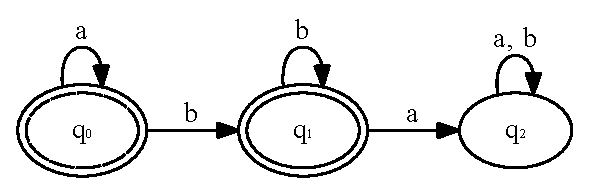
\includegraphics{graph2.eps}
\caption{Automaatin tilakaavio}
\end{figure}

Siirtymäfunktio voidaan myös kuvata taulukkona:
\\
\begin{center}
\begin{tabular} {c | c c c}
& $q_0$ & $q_1$ & $q_2$ \\
\hline
$a$ & $q_0$ & $q_2$ & $q_2$ \\
$b$ & $q_1$ & $q_1$ & $q_2$ \\
\end{tabular}
\end{center}

Tämä kone hyväksyy vain merkkijonot, jotka ovat muotoa $a^nb^m$, $n, m \in \mathbb{N}$.

Jos syötteeksi annetaan esimerkiksi merkkijono aaabb, suoritus etenisi seuraavasti:\\

\begin{center}
\begin{tabular}{r c l }
Tila & Merkki & Jäljellä oleva syöte \\
$q_0$ & a & aabb \\
$q_0$ & a & abb \\
$q_0$ & a & bb \\
$q_0$ & b & b \\
$q_1$ & b & \\
$q_1$ & & \\
\end{tabular}
\end{center}

Koska $q_1 \in F$, kone antaa tulokseksi 'kyllä'.

Toisaalta jos syötteenä olisi aba, suoritus etenisikin seuraavasti:
\\
\begin{center}
\begin{tabular}{r c l }
Tila & Merkki & Jäljellä oleva syöte \\
$q_0$ & a & ba \\
$q_0$ & b & a \\
$q_1$ & a &  \\
$q_2$ & & \\
\end{tabular}
\end{center}

Koska $q_2 \notin F$, kone antaisi tulokseksi 'ei'.
\end{example}

\begin{teor}
Olkoon $M$ esimerkissä 3 määritelty automaatti. \\ $L(M) = \{a^nb^m | n, m \in \mathbb{N}\}$.
\begin{proof}
Olkoon sana $w \in \Sigma^*$. Jos $w \in L(M)$, niin automaatti selvästi palauttaa tuloksen 'kyllä'. Jos $w \notin L(M)$, niin sen täytyy sisältää ainakin yksi $ba$-pari. Tämä riittää siirtämään automaatin mistä hyvänsä tilasta tilaan $q_2$. Mikään merkki ei siirrä automaattia tilasta $q_2$ mihinkään muuhun tilaan, joten suorituksen päätyttyä kone on edelleen tilassa $q_2$, ja palauttaa siis tulokseksi 'ei'.
\qedhere
\end{proof}
\end{teor}


Äärellisillä automaateilla on kuitenkin monia rajoitteita. On runsaasti esimerkkejä ongelmista, jotka intuitiivisesti olisivat ratkaistavissa jollaking algoritmilla, mutta joita ei voi laskea äärellisen automaatin avulla. Tällaisia ongelmia ovat esimerkiksi 'Onko annettu suljelauseke oikein muodostettu?' tai 'Onko merkkijono muotoa $a^nb^n$?'. Onkin selvää, että äärelliset automaatit eivät ole riittävän yleisiä toteuttaakseen kaikkia algoritmeja.

\begin{teor}
Ei ole olemassa äärellistä automaattia $M$, joka tunnistaa kielen $L = \{a^nb^n | n \geq 0\}$.
\begin{proof}
Olkoon $M$ äärellinen automaatti, jolla on $n$ tilaa. Mikä tahansa merkkijono, jonka pituus on vähintään $n$ aiheuttaa sen, että jokin koneen tiloista toistetaan. Merkitään tätä tilaa $S$. Siirtymä tämän tilan ensimmäisestä esiintymästä toiseen vastaa jotakin käsitellyn merkkijonon osaa. Olkoon tämä osa $y$. Jos kone on tilassa $S$ ja se saa syötteekseen $y$:n, päätyy se taas tilaan $S$. Tästä seuraa, että jos automaatti hyväksyy sanan $w = xyz$, täytyy sen hyväksyä sana $xy^iz, i \geq 0$.

Sovelletaan tätä nyt kielen $L$ tapaukseen. Olkoon $w = a^mb^m, m > n$. Tällöin on olemassa sellainen jako $i + j + k = m, j > 0$, että kone $M$ tunnistaa sanat $a^ia^{j*p}a^kb^m, p \in \mathbb{N}$. Näistä kuitenkin vain yksi kuuluu kieleen $L$, joten $L(M) \neq L$.
\qedhere
\end{proof}
\end{teor}

\section{Rekisterikoneet}
Shepherdsonin ja Sturgisin rekisterikoneet ovat rakenteellisesti hyvin yksinkertaisia. Koneella on $R$ rekisteriä, joista kukin muistaa yhden luonnollisen luvun. Rekisterin $n$ arvoon viitataan merkinnällä $\bar{n}$. Suoritettava algoritmi esitetään numeroituna luettelona, joka koostuu hyvin yksinkertaisista komennoista. Merkitään näitä komentoja $\hat{1}$, $\hat{2}$, \dots , $\hat{M}$. Algoritmin alkuarvot on tallennettu rekistereihin. Rekisterikone tunnistaa kolme erilaista komentoa: $(n,j)$, $(n,j,k)$ sekä lopetuskomennon $\hat{M}$. Kahden ensimmäisen komennon merkitykset ovat:

\begin{tabular}{c l}
$(n, j)$ & Lisää 1 rekisteriin n ja siirry komentoon j. \\
$(n, j, k)$ & Jos $\bar{n} > 0$, vähennä 1 rekisteristä n ja siirry komentoon j; \\
& muutoin siirry komentoon k.\\
\end{tabular}


Näillä sinänsä yksinkertaisilla säännöillä on mahdollista suorittaa monimutkaisiakin laskutoimituksia.

\begin{example}
Määritellään rekisterikone joka suorittaa yhteenlaskun.
\\
\begin{math} \\
R = 2, M = 3 \\
\hat{1} (2,2,3) \\
\hat{2} (1,1) \\
\hat{3} \text{Seis}\\
\end{math}
\\
Olkoon rekisterien arvot alkutilanteessa $(3, 2)$. Ohjelman suoritus etenisi seuraavalla tavalla:\\ \\
\\
\begin{figure}[H]
\begin{center}
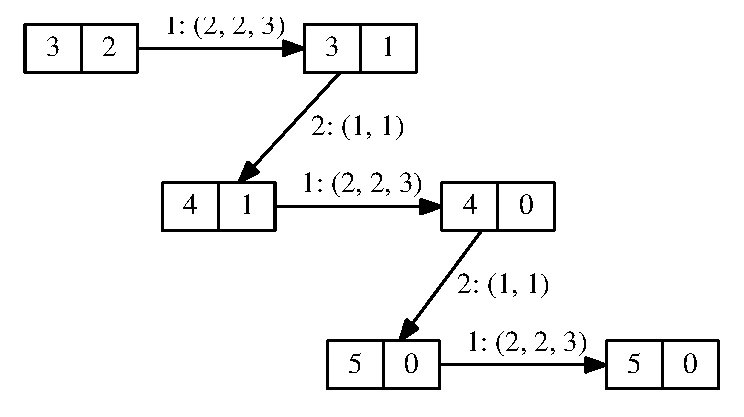
\includegraphics{graph3.eps}
\caption{Esimerkki rekisterikoneen toiminnasta}
\end{center}
\end{figure}


\end{example}

% Esimerkkejä muista ohjelmista.


\section{Turingin koneet}
Turing kone on ensimmäinen tunnettu muodollinen kone. Alan Turing esitteli sen vuonna 1937, kun käytti sitä apuvälineenä ratkaistakseen David Hilbertin vuonna 1928 esittämän päätösongelman.
Turingin koneet poikkeavat rakenteellisesti rekisterikoneista huomattavasti ja muistuttavat enemmänkin äärellisiä tilakoneita. Muodollisesti määriteltynä Turingin koneella on seitsemän komponenttia $(Q, \Sigma, \Gamma, \delta, q_0, B, F)$, jossa

\begin{itemize}
\item äärellinen tilajoukko $Q$
\item nauha-aakkosto $\Gamma$
\item syöteaakkosto $\Sigma \subset \Gamma$
\item siirtymäfunktio $\delta : Q \times \Gamma \rightarrow Q \times \Gamma \times \{L,R\}$
\item alkutila $q_0$
\item 'tyhjä' nauhasymboli $B \in \Gamma - \Sigma$
\item hyväksyvien tilojen joukko $F \subseteq Q.$
\end{itemize}

Turingin koneiden ajatellaan käsittelevän kaksisuuntaisesti ääretöntä nauhaa, jonka jollekin äärelliselle alueelle on kirjoitettu symboleja. Muu nauha sisältää vain symbolia $B$ ('blank' eli tyhjä).
Turingin koneet toimivat kuten äärelliset automaatit lukuun ottamatta kahta merkittävää eroa. Ne voivat siirtyä nauhaa sekä eteen- että taaksepäin, ja ne voivat muuttaa nauhan sisältöä.

Alkutilanteessa kone aloittaa syötteen vasemmasta reunasta, tilassa $q_0 \in Q$. Kone lukee yhden merkin ja päättää sen perusteella mihin tilaan siirtyä, minkä merkin kirjoittaa nauhalle luetun merkin tilalle ja siirtyäkö oikealle vai vasemmalle. Suoritus päättyy vasta, kun siirtymäfunktio $\delta$ palauttaa arvon $\emptyset$. Sen jälkeen verrataan senhetkistä tilaa joukkoon $F$ kuten äärellisten automaattien tapauksessa.


%Esimerkki Turingin koneen toiminnasta, ehkä määritellään kone joka tekee jotain, annetaan parin askeleen esimerkki
\begin{example}
Olkoon $M$ Turingin kone siten, että\\$M = (\{q_0, q_a, q_b, q_r, q_e\}, \{a, b\}, \{a, b, B\}, \delta, q_0, B, \{s\})$ missä $\delta$ toimii seuraavan taulukon mukaisesti:

\begin{tabular}{r | l l l}
& a & b & B \\
\hline
$q_0$ & $(q_a, B, R)$ & $(q_e, b, R)$ & $\emptyset$ \\
$q_a$ & $(q_a, a, R)$ & $(q_a, b, R)$ & $(q_b, B, L)$ \\
$q_b$ & $(q_e, a, R)$ & $(q_r, B, L)$ & $(q_e, B, R)$\\
$q_r$ & $(q_r, a, L)$ & $(q_r, b, L)$ & $(q_0, B, R)$\\
$q_e$ & $\emptyset$ & $\emptyset$ & $\emptyset$ \\ 
\end{tabular}

Tällä tavoin määritelty Turingin kone tunnistaa kielen $\{a^nb^n | n \geq 0\}$, jota äärelliset automaatit eivät pysty tunnistamaan.

\end{example}

\section{Funktioiden esittäminen muodollisella koneella}

Useimmissa tapauksissa ei riitä, että algoritmi tuottaa kyllä/ei -vastauksen, vaan algoritmin toivotaan tuottavan esimerkiksi laskutoimituksen tuloksen. Näissä tapauksissa ei ole tärkeää se, missä tilassa kone on lopettaessaan suorituksen, vaan se, mitä rekistereissä tai nauhalla on. Lopetustilan tarkastelu ei tällaisissa tapauksissa ole tarpeellista, vaan voimme pitää kaikkia lopetustiloja hyväksyttävinä.

Se, miten algoritmi palauttaa vastauksen, on sopimuskysymys. Turingin koneen tapauksessa vastaus luetaan nauhalta suorituksen päätyttyä, ja rekisterikoneen tapauksessa tulos tallennetaan yleensä rekisteriin yksi.

\section{Rekisterikoneiden ja Turingin koneiden\\ välinen yhteys}

Vaikka Turingin koneet ja rekisterikoneet ovat rakenteellisesti hyvin erilaisia, ovat ne kuitenkin osoittautuneet laskukyvyltään ekvivalenteiksi. Jos ongelma on ratkaistavissa rekisterikoneella, se on myös ratkaistavissa Turingin koneella ja päinvastoin. Se, että näinkin erilaiset koneet ovat yhtä ilmaisuvoimaisia, viittaa siihen, että olemme lähestymässä käyttökelpoista tapaa määritellä laskettavuuden käsite. Laskettavuus samaistetaankin usein laskettavuuteen Turingin koneilla.

\begin{mydef}
Olkoon sana $w = \Sigma^*$ jonka pituus on $n$. Olkoon $w_i$ sanan $i$:des merkki, ja olkoon kuvaus $f: \Sigma \rightarrow \mathbb{N}$ injektio. Sanan $w$ \emph{alkulukukoodaus} on bijektio $p: \Sigma^* \rightarrow \mathbb{N}$ missä $$p(w) = \prod_{i=1}^{n} p_i^{f(w_i)}$$ ja $p_i$ on $i$:s alkuluku.
\end{mydef}
Kuvauksen $f$ valinta ei ole tärkeää, kunhan samassa yhteydessä käytetään aina samaa kuvausta. Mikäli kuvausta ei erikseen määritellä, oletetaan yleensä sen kuvaavan aakkoston positiivisiin kokonaislukuihin samassa järjestyksessä missä merkit lueteltiin.
\begin{example}
Olkoon $\Sigma = {a, b, c}$ ja $w = abac$. $w$:n alkulukukoodaus olisi tässä tapauksessa $p(w) = p_1^{f(a)} \times  p_2^{f(b)} \times  p_3^{f(a)} \times  p_4^{f(c)} = 2^1\times3^2\times5^1\times7^3 = 30870$.
\end{example}

\begin{teor}
Olkoon $f$ k:n muuttujan funktio. Funktio $f$ on laskettavissa rekisterikoneella jos ja vain jos se on laskettavissa Turingin koneella.
\begin{proof}
Osoitetaan ensin, että annetun Turingin koneen $M$ toimintaa voidaan simuloida sopivasti rakennetulla rekisterikoneella. Jos tämä pitää paikkansa, mikä tahansa Turingin koneella ratkaistavissa oleva ongelma voidaan ratkaista myös rekisterikoneella tarvittaessa simuloimalla ko. Turingin koneen toimintaa. Tämän jälkeen osoitetaan, että sama pätee myös toiseen suuntaan.

Olkoon $M$ Turingin kone. $M$:n tämän hetkinen konfiguraatio koostuu nauhan sisällöstä, tällä hetkellä tutkittavasta symbolista sekä koneen tilasta. Vaikka nauha on ääretön, voimme mallintaa sitä äärellisenä, sillä vain äärellisen moni merkki on epätyhjä. Nauha-aakkosto on äärellinen, joten nauhan sen hetkinen tila voidaan ilmaista yhtenä lukuna alkulukukoodauksella. Tallennetaan tämä ensimmäiseen rekisteriin, jota ei käytetä syötteen vastaanottamiseen. Seuraavaan rekisteriin tallennetaan tutkittavan merkin sijaintia vastaava luonnollinen luku, ja sitä seuraavaan koneen tämän hetkistä tilaa vastaava luku.
\begin{figure}[H]
\centering
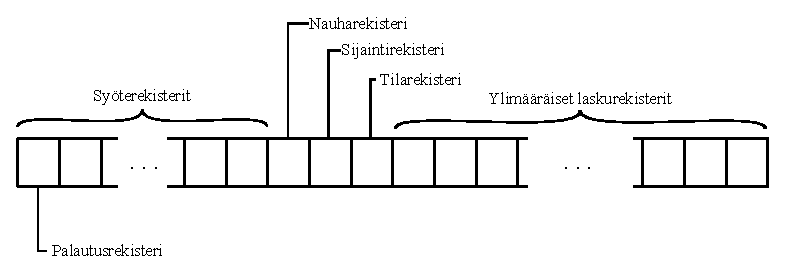
\includegraphics{graph5.eps}
\caption{Rekistereiden valinta}
\end{figure}
Tämän jälkeen voidaan kuvailla rekisterikoneen varsinainen toiminta. Jokaista paria $(q_i, a), q_i \in Q, a \in \Gamma$ kohden on komentosarja, joka muokkaa rekistereitä niin, että se vastaa sitä mitä koneessa M olisi tapahtunut. Jos $\delta(q_i, a) = \emptyset$ koneen tulisi pysähtyä, mutta tässä tapauksessa tulee ensin purkaa ja kopioida nauharekisterin sisältö tulosrekisteriin. Jos $\delta(q_i, a) = (q_j, b, L)$ tai $(q_j, b, R)$ tulee kirjoittaa komentosarja joka muokkaa kolmea tilarekisteriä koneen M tavoin. Tällaisten komentosarjojen tuottaminen täsmällisesti on varsin työlästä, mutta ei kovin vaikeaa.
% Esimerkki tästä?

Näiden lisäksi joudumme myös määrittelemään tällaisen koneen aloitustilan. Tämä tapahtuu asettamalla syötenauhaa vastaava luku nauharekisteriin, 1 käsiteltävän merkin numeroksi sekä 0 koneen tilaksi.

Käänteisesti tulee rakentaa sellainen Turingin kone, joka pystyy simuloimaan annetun rekisterikoneen toimintaa. Olkoon rekisterikoneella $R$ rekisteriä. Tällöin tallennetaan yhden rekisterin sisälltö koodattuna joka $R$:nteen muistipaikkaan valitusta rajasta eteenpäin. Esimerkiksi jos $R = 2$, joka toinen nauhan muistipaikka kuuluisi rekisteriin 1 ja joka toinen rekisteriin 2. Rekisterien sisältö voidaan koodata nauhalle monin eri tavoin. Yksinkertaisuuden vuoksi käytetään tässä unaarista lukujärjestelmää.

\begin{figure}[H]
\begin{center}
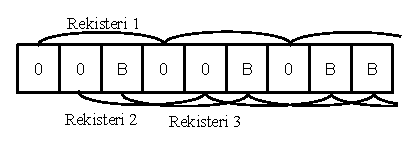
\includegraphics{graph4b.eps}
\caption{Rekisterien sijoittelu nauhalle tapauksessa R = 3. Rekistereissä ovat kuvattuna arvot $(3, 2, 0)$, nauha on muualla tyhjä.}
\end{center}
\end{figure}

Ensimmäiseksi annettu syöte tulee muuntaa edellä kuvattuun muotoon. Tarvittavan aliohjelman teko on helppoa.

Sen jälkeen kirjoitetaan aliohjelmat, jotka suorittavat samat toiminnot kuin $(n, j)$ ja $(n, j, k)$. Kannattanee pitää tarkoitukseen varattua merkkiä rekisterialueen vasemmalla puolen, jotta se löytyy helpommin. Tässä tarkoitukseen käytetään merkkiä 1. Olkoon Turingin koneen lukupää tällä merkillä seuraavia aliohjelmia varten, ja olkoon se komentoa $(n, j)$ vastaavassa tilassa. Aluksi kone siirtyy $n-1$ merkkiä oikealle, jolloin se saavutta rekisteriä n vastaavan alueen. Tämän jälkeen se siirtyy oikealle $R$:n pituisin askelin, kunnes se löytää tyhjän merkin. Kone asettaa sen 0:ksi, palaa takaisin vasemmalle merkin 1 luokse ja muuttaa tilansa rekisterikoneen komentoa \^j vastaavaksi. Tällä tavoin rekisterin n arvoa on kasvatettu yhdellä. Olkoon kone nyt komentoa $(n, j, k)$ vastaavassa tilassa. Kone siirtyy ensin $n - 1$ merkkiä oikealle. Jos sillä kohdalla oleva merkki on tyhjä, palataan kohtaan 1 ja siirrytään rekisterikoneen komentoa \^k vastaavaan tilaan. Jos merkki ei ollut tyhjä, siirrymme oikealle R:n pituisin askelin kunnes löydämme tyhjän merkin. Siirrymme $R$ merkkiä vasemmalle, merkitsemme sen tyhjäksi, siirrymme takaisin merkin 1 luo ja siirrymme komentoa \^j vastaavaan tilaan.

Kun komento 'Seis' saavutetaan, ensimmäisen rekisterin sisältö talletetaan ja muu nauha tyhjennetään.

\qedhere

Tässä todistuksessa havaitaan myös, että mikäli algoritmin suoritus yhdellä koneella ei koskaan pääty, myöskään toisella koneella simuloitu suoritus ei koskaan pääty.

\end{proof}
\end{teor}

\appendix

\section{Lähteet}
J. Truss: Discrete Mathematics For Computer Scientists, Addison-Wesley, 1999.

\end{document}